\chapter{Angular Resolution: Baselines, Diffraction, and Pixel Sampling}

The ability of an astronomical telescope to distinguish fine spatial details on the sky is governed by four interconnected physical and geometric principles:
\begin{enumerate}[leftmargin=2em]
	\item \textbf{Interferometric baseline geometry:} The physical straight-line chord separation between distributed collecting elements.
	\item \textbf{Telescope optics and focal scaling:} The geometric mapping of angular angles on the sky to linear physical displacements in the focal plane.
	\item \textbf{Diffraction wave optics:} The fundamental wave limit imposed by Fraunhofer diffraction through a finite circular aperture (the Airy disk and Rayleigh criterion).
	\item \textbf{Detector pixelization and sampling:} The matching between physical pixel sizes and the optical point spread function via the Nyquist--Shannon sampling theorem, along with atmospheric seeing and Adaptive Optics ($\mathrm{AO}$).
\end{enumerate}

\section{Interferometric Baselines: Chord Distance Between Ground Stations}

In Very Long Baseline Interferometry (VLBI) and connected-element radio interferometers (such as the GMRT or ALMA), the physical separation between two antennas defines the interferometer \emph{baseline}.

\subsection{Central Angle on a Spherical Earth}

Let two observatories be located at geodetic coordinates $(\phi_1, \lambda_1)$ and $(\phi_2, \lambda_2)$ on a spherical Earth of mean radius $R_E \approx 6371.0\,\mathrm{km}$. In the Earth-centered Cartesian coordinate frame:
\begin{equation}
	\hat{\mathbf r}_i = \begin{pmatrix} \cos\phi_i\cos\lambda_i \\ \cos\phi_i\sin\lambda_i \\ \sin\phi_i \end{pmatrix}, \qquad i \in \{1, 2\}.
	\label{eq:earth_station_vector}
\end{equation}

\begin{figure}[htbp]
	\centering
	\begin{minipage}[c]{0.38\textwidth}
		\begin{equation}
		\hat{\mathbf{r}}_{\rm geodetic} = 
		\begin{pmatrix}
		\cos\phi\cos\lambda\\
		\cos\phi\sin\lambda\\
		\sin\phi
		\end{pmatrix}
		\end{equation}
	\end{minipage}
	\hfill
	\begin{minipage}[c]{0.58\textwidth}
		\centering
		\begin{tikzpicture}[
			scale=1.4, 
			x={(-0.6cm,-0.3cm)}, 
			y={(0.9cm,-0.2cm)}, 
			z={(0cm,0.95cm)},
			>=Stealth
			]
			% Parameters
			\def\alphaDeg{45}
			\def\deltaDeg{35}
			\def\R{2.0}
			\pgfmathsetmacro{\Rproj}{\R*cos(\deltaDeg)}
			
			% Coordinates
			\coordinate (O)  at (0,0,0);
			\coordinate (X)  at (3.5,0,0);
			\coordinate (Y)  at (0,2.6,0);
			\coordinate (Z)  at (0,0,2.6);
			
			\coordinate (P)  at ({\Rproj*cos(\alphaDeg)}, {\Rproj*sin(\alphaDeg)}, {\R*sin(\deltaDeg)}); 
			\coordinate (PP) at ({\R*cos(\alphaDeg)}, {\R*sin(\alphaDeg)}, 0);
			
			% Colors
			\definecolor{axisColor}{HTML}{2B3A42}
			\definecolor{vectorColor}{HTML}{E74C3C}
			\definecolor{arcColor}{HTML}{0D9488}
			\definecolor{guideColor}{HTML}{94A3B8}
			\definecolor{sphereGrid}{HTML}{CBD5E1}
			
			% Background
			\begin{scope}
				\draw[sphereGrid, line width=0.8pt] (O) circle (1.08*\R cm);
				\draw[sphereGrid!80, dashed, line width=0.5pt] plot[domain=0:360, variable=\t, smooth] 
				({\R*cos(\t)}, {\R*sin(\t)}, 0);
				\draw[sphereGrid!70, dotted, line width=0.5pt] plot[domain=0:360, variable=\t, smooth] 
				({\Rproj*cos(\t)}, {\Rproj*sin(\t)}, {\R*sin(\deltaDeg)});
			\end{scope}
			
			% Axes
			\draw[->, axisColor, line width=1.1pt] (O) -- (X) node[below left, font=\bfseries] {$\boldsymbol{x}$};
			\draw[->, axisColor, line width=1.1pt] (O) -- (Y) node[right, font=\bfseries] {$\boldsymbol{y}$};
			\draw[->, axisColor, line width=1.1pt] (O) -- (Z) node[above, font=\bfseries] {$\boldsymbol z$};
			\node[axisColor, left=2pt, font=\bfseries] at (O) {$O$};
			
			% Reference line to P'
			\draw[dashed, guideColor, line width=0.9pt] (O) -- (PP);
			
			% Radius vector r_eq
			\draw[->, vectorColor, line width=1.8pt] (O) -- (P) 
			node[midway, above left, color=axisColor] {$\hat{\mathbf{r}}$};
			
			% Spherical Arc \lambda (Equator)
			\draw[->, arcColor, line width=1.5pt] plot[domain=0:\alphaDeg, variable=\t, smooth]
			({\R*cos(\t)}, {\R*sin(\t)}, 0);
			\node[arcColor, font=\bfseries] at ({1.15*\R*cos(\alphaDeg/2)}, {1.15*\R*sin(\alphaDeg/2)}, -0.1) {$\lambda$};
			
			% Spherical Arc \phi (Meridian)
			\draw[->, arcColor, line width=1.5pt] plot[domain=0:\deltaDeg, variable=\t, smooth]
			({\R*cos(\t)*cos(\alphaDeg)}, {\R*cos(\t)*sin(\alphaDeg)}, {\R*sin(\t)});
			\node[arcColor, font=\bfseries] at ($(PP)!0.5!(P)+(0.25,0.05,0)$) {$\phi$};
			
			% Points P and P'
			\fill[vectorColor] (P) circle (1.2pt) node[above right=1pt, font=\bfseries, color=axisColor] {$P$};
			\fill[arcColor!80!black] (PP) circle (1.2pt) node[below right=1pt, font=\bfseries, color=axisColor] {$P'$};
		\end{tikzpicture}
	\end{minipage}
	\caption{Geodetic coordinate definition on a spherical Earth with latitude $\phi$ and longitude $\lambda$.}
	\label{fig:earth_geodetic_vector}
\end{figure}

The angular separation $\gamma$ subtended by the two stations at the Earth's center is determined by their dot product:
\begin{align}
	\cos\gamma &= \begin{pmatrix} \cos\phi_1\cos\lambda_1 & \cos\phi_1\sin\lambda_1 & \sin\phi_1 \end{pmatrix} \begin{pmatrix} \cos\phi_2\cos\lambda_2 \\ \cos\phi_2\sin\lambda_2 \\ \sin\phi_2 \end{pmatrix} \notag\\
	&= \sin\phi_1\sin\phi_2 + \cos\phi_1\cos\phi_2\cos(\lambda_2-\lambda_1).
	\label{eq:earth_central_angle}
\end{align}

\subsection{Straight-Line Chord Baseline Geometry}

The straight-line (shortest distance in 3D) between two stations is given by measuring the \emph{chord distance} $C$ passing through the Earth's interior:

\begin{figure}[htbp]
    \centering
    \begin{minipage}[c]{0.42\textwidth}
        
\includegraphics[width=\linewidth]{obs_vlbi_ggos_web_v2-1024x949.png}
    \end{minipage}
    \hfill
    \begin{minipage}[c]{0.54\textwidth}
    \centering
    \begin{tikzpicture}[scale=1.0, >=Stealth]
    % Define the radius and angle
    \def\RE{3.6}
    \def\gammaangle{60}

    % Define coordinates rotated by 90 degrees
    \coordinate (O) at (0,0);
    \coordinate (A) at (90+\gammaangle/2:\RE);
    \coordinate (B) at (90-\gammaangle/2:\RE);
    
    % M is the midpoint of the chord for the perpendicular bisector
    \coordinate (M) at (90:{\RE*cos(\gammaangle/2)});

    % Draw the top arc
    \draw[thick] (0:\RE) arc (0:180:\RE);

    % Draw the radii
    \draw[thick] (O) -- (A) node[midway, left=4pt] {$R_E$};
    \draw[thick] (O) -- (B) node[midway, right=4pt] {$R_E$};

    % Draw the full chord
    \draw[thick, blue] (A) -- (B);

    % Draw the perpendicular bisector
    \draw[thick, dashed, red] (O) -- (M);

    % Right angle marker at the intersection
    \draw (M) ++(0,-0.2) -- ++(0.2,0) -- ++(0,0.2);

    % Label the half-chord distances using braces
    \draw[decorate, decoration={brace, amplitude=5pt, raise=2pt}, thick]
         (A) -- (M) node[midway, above=10pt] {$R_E \sin(\gamma/2)$};
    \draw[decorate, decoration={brace, amplitude=5pt, raise=2pt}, thick]
         (M) -- (B) node[midway, above=10pt] {$R_E \sin(\gamma/2)$};

    % Draw and label the split angles
    \pic [draw, thick, "$\frac{\gamma}{2}$", angle eccentricity=1.6, angle radius=0.9cm] {angle = M--O--A};
    \pic [draw, thick, "$\frac{\gamma}{2}$", angle eccentricity=1.6, angle radius=0.9cm] {angle = B--O--M};

    % Mark and label the points
    \fill (O) circle (2pt) node[below=2pt] {$O$};
    \fill (A) circle (2pt) node[above left] {$P_1$};
    \fill (B) circle (2pt) node[above right] {$P_2$};
    \fill (M) circle (1.5pt) node[below right=1pt] {$M$};
    \end{tikzpicture}
    \end{minipage}
    \caption{Global VLBI network (left) and the chord baseline geometry $C = 2R_E\sin(\gamma/2)$ through the Earth's interior (right).}
    \label{fig:vlbi_chord_geometry}
\end{figure}

The straight-line chord distance is therefore:
\begin{keyresult}
	\begin{equation}
		C = 2R_E\sin\left(\frac{\gamma}{2}\right) = R_E\sqrt{2(1-\cos\gamma)}.
		\label{eq:chord_baseline_formula}
	\end{equation}
\end{keyresult}

\subsection{Derivation of the Baseline Interferometer Angular Resolution Limit}

To understand how an interferometer synthesizes high angular resolution from two antennas separated by a physical baseline $B$, consider two distinct astronomical point sources on the sky, \textbf{Source 1} and \textbf{Source 2}, observed simultaneously at observing wavelength $\lambda$.

\begin{figure}[htbp]
\centering
\begin{tikzpicture}[scale=1.15, >=Stealth]
    \def\B{6.0}
    \def\thOne{20}
    \def\thTwo{42}
    \def\rayLen{5.2}
    
    \coordinate (A1) at (0,0);
    \coordinate (A2) at (\B,0);
    
    % Normal lines
    \draw[dashed, gray!60, thick] (A1) -- (0, 4.8) node[above, gray!80!black] {Normal};
    \draw[dashed, gray!60, thick] (A2) -- (\B, 4.8) node[above, gray!80!black] {Normal};
    
    % Source 1 directions (coming from upper right at angle thOne to normal)
    \pgfmathsetmacro{\sOneX}{\rayLen*sin(\thOne)}
    \pgfmathsetmacro{\sOneY}{\rayLen*cos(\thOne)}
    \coordinate (S1_A1) at (\sOneX, \sOneY);
    \coordinate (S1_A2) at ({\B + \sOneX}, \sOneY);
    
    % Source 2 directions (coming from upper right at angle thTwo to normal)
    \pgfmathsetmacro{\sTwoX}{\rayLen*sin(\thTwo)}
    \pgfmathsetmacro{\sTwoY}{\rayLen*cos(\thTwo)}
    \coordinate (S2_A1) at (\sTwoX, \sTwoY);
    \coordinate (S2_A2) at ({\B + \sTwoX}, \sTwoY);
    
    % Intersection points W1 and W2 on ray A1 from wavefronts starting at Antenna 2 (A2)
    \pgfmathsetmacro{\wOneX}{\B*sin(\thOne)*sin(\thOne)}
    \pgfmathsetmacro{\wOneY}{\B*sin(\thOne)*cos(\thOne)}
    \coordinate (W1) at (\wOneX, \wOneY);
    
    \pgfmathsetmacro{\wTwoX}{\B*sin(\thTwo)*sin(\thTwo)}
    \pgfmathsetmacro{\wTwoY}{\B*sin(\thTwo)*cos(\thTwo)}
    \coordinate (W2) at (\wTwoX, \wTwoY);
    
    % Incoming rays for Source 1 (Red)
    \draw[->, very thick, red!80!black] (S1_A1) -- (A1);
    \draw[->, very thick, red!80!black] (S1_A2) -- (A2);
    
    % Incoming rays for Source 2 (Blue)
    \draw[->, very thick, blue!80!black] (S2_A1) -- (A1);
    \draw[->, very thick, blue!80!black] (S2_A2) -- (A2);
    
    % Wavefronts from Antenna 2 (A2) hitting rays at Antenna 1 at exact 90 degrees
    \draw[dashed, line width=1.1pt, red!80!black] (A2) -- (W1);
    \draw[dashed, line width=1.1pt, blue!80!black] (A2) -- (W2);
    
    % Right angle markers at W1 and W2 (exact 90-degree square markers)
    \pgfmathsetmacro{\sqSize}{0.28}
    \draw[thick, red!80!black] 
        ($(W1) + ({\sqSize*cos(\thOne)}, {-\sqSize*sin(\thOne)})$) -- 
        ++({-\sqSize*sin(\thOne)}, {-\sqSize*cos(\thOne)}) -- 
        ($(W1) + ({-\sqSize*sin(\thOne)}, {-\sqSize*cos(\thOne)})$);
        
    \draw[thick, blue!80!black] 
        ($(W2) + ({\sqSize*cos(\thTwo)}, {-\sqSize*sin(\thTwo)})$) -- 
        ++({-\sqSize*sin(\thTwo)}, {-\sqSize*cos(\thTwo)}) -- 
        ($(W2) + ({-\sqSize*sin(\thTwo)}, {-\sqSize*cos(\thTwo)})$);
        
    % Path lags along ray entering Antenna 1
    \draw[line width=3.0pt, red!80!black] (W1) -- (A1);
    \node[left=4pt, red!80!black, font=\bfseries] at ($(W1)!0.5!(A1)$) {$\Delta L_1 = B\sin\theta_1$};
    
    \draw[line width=3.0pt, blue!80!black] (W2) -- (A1);
    \node[right=4pt, blue!80!black, font=\bfseries] at ($(W2)!0.6!(A1)$) {$\Delta L_2 = B\sin\theta_2$};
    
    % Baseline line
    \draw[line width=1.6pt, ink] (A1) -- (A2) node[midway, below=6pt] {\textbf{Baseline} $B$};
    \fill[astroblue] (A1) circle (3pt) node[below left=2pt] {\textbf{Antenna 1} ($A_1$)};
    \fill[astroblue] (A2) circle (3pt) node[below right=2pt] {\textbf{Antenna 2} ($A_2$)};
    
    % Angle arcs at A2
    \draw[->, thick, red!80!black] (\B, 2.2) arc (90:{90-\thOne}:2.2) node[midway, above] {$\theta_1$};
    \draw[->, thick, blue!80!black] (\B, 3.2) arc (90:{90-\thTwo}:3.2) node[midway, above right] {$\theta_2$};
    
    % Angle arcs at A1
    \draw[->, thick, red!80!black] (0, 2.2) arc (90:{90-\thOne}:2.2) node[midway, above] {$\theta_1$};
    \draw[->, thick, blue!80!black] (0, 3.2) arc (90:{90-\thTwo}:3.2) node[midway, above right] {$\theta_2$};
    
    % Source labels at top
    \node[red!80!black, right=2pt, font=\bfseries] at (S1_A2) {Source 1};
    \node[blue!80!black, right=2pt, font=\bfseries] at (S2_A2) {Source 2};
\end{tikzpicture}
\caption{Geometric optical path delays for two distinct sources observed by a two-element interferometer of baseline $B$. Wavefronts from Antenna 2 ($A_2$) strike the rays entering Antenna 1 ($A_1$) at right angles ($90^\circ$), defining the respective geometric lags $\Delta L_1 = B\sin\theta_1$ and $\Delta L_2 = B\sin\theta_2$.}
\label{fig:interferometer_two_sources}
\end{figure}

Let the directions to the two sources make angles $\theta_1$ and $\theta_2$ with respect to the baseline normal:
\begin{enumerate}
	\item \textbf{Geometric Path Lag for Source 1:} A plane wavefront from Source 1 arrives at Antenna 2 before Antenna 1. The extra path distance that the light must travel to reach Antenna 1 is:
	\begin{equation}
		\Delta L_1 = B\sin\theta_1.
		\label{eq:path_lag_source_1}
	\end{equation}
	\item \textbf{Geometric Path Lag for Source 2:} Similarly, a plane wavefront from Source 2 arrives at angle $\theta_2$, resulting in a geometric path lag to Antenna 1 of:
	\begin{equation}
		\Delta L_2 = B\sin\theta_2.
		\label{eq:path_lag_source_2}
	\end{equation}
	\item \textbf{Differential Path Difference Between the Two Sources:} The net difference in path delay between the signals arriving from the two sources across the baseline is:
	\begin{equation}
		\Delta(\Delta L) = \Delta L_2 - \Delta L_1 = B\left(\sin\theta_2 - \sin\theta_1\right).
		\label{eq:diff_path_difference}
	\end{equation}
	For closely spaced sources on the sky, let $\theta = \theta_2 - \theta_1$ denote their mutual angular separation. Using the small-angle approximation ($\sin\theta_2 - \sin\theta_1 \approx \theta_2 - \theta_1 = \theta$ for angles near the normal):
	\begin{equation}
		\Delta(\Delta L) = B\left(\sin\theta_2 - \sin\theta_1\right) \approx B\theta.
		\label{eq:diff_path_approx}
	\end{equation}
	\item \textbf{Interferometric Resolution Criterion:} In a radio/optical interferometer, incoming wavefronts are correlated to produce sinusoidal interference fringe patterns. For the interferometer to cleanly resolve (distinguish) Source 1 from Source 2, the fringe pattern of Source 2 must shift relative to that of Source 1 by at least \textbf{one full interference fringe cycle} (corresponding to a full phase shift of $\Delta\phi = 2\pi$), which requires an extra path difference of exactly one full wavelength $\lambda$:
	\begin{equation}
		B\left(\sin\theta_2 - \sin\theta_1\right) = B\theta = \lambda.
		\label{eq:interferometer_resolution_condition}
	\end{equation}
\end{enumerate}

Solving Eq.~\eqref{eq:interferometer_resolution_condition} for the limiting angular resolution $\theta_{\rm res}$:
\begin{keyresult}
	\begin{equation}
		\theta_{\rm res} = \frac{\lambda}{B}\quad [\text{radians}] = \frac{\lambda}{B} \times \frac{180 \times 3600}{\pi}'' = 206{,}265\left(\frac{\lambda}{B}\right)\quad [\text{arcseconds}].
		\label{eq:interferometric_resolution_formula}
	\end{equation}
\end{keyresult}
This fundamental equation demonstrates that interferometric resolution depends solely on the ratio of the observing wavelength $\lambda$ to the baseline separation $B$, allowing distributed arrays to synthesize effective apertures thousands of kilometers wide.

\subsection{Worked Example: Interferometric Resolution for the GMRT to Ooty Baseline}

The baseline length $B = C$ determines the synthesized angular resolution as derived above:
\begin{equation}
	\theta \simeq \frac{\lambda}{B}.
	\label{eq:interferometric_res_approx}
\end{equation}

\begin{example}[Interferometry Between GMRT and Ooty Radio Telescope]
	The coordinates $(\phi,\lambda)$ of the Giant Metrewave Radio Telescope (GMRT, Khodad) and Ooty Radio Telescope (ORT) are:
	\[
	\begin{aligned}
		\text{GMRT}:&\quad (19.09^\circ\text{N},\,74.05^\circ\text{E}),\\
		\text{Ooty}:&\quad (11.38^\circ\text{N},\,76.66^\circ\text{E}).
	\end{aligned}
	\]
	\begin{enumerate}
		\item \textbf{Baseline Distance:} Using Eq.~\eqref{eq:earth_central_angle}:
		\[
		\cos\gamma = \sin(19.09^\circ)\sin(11.38^\circ) + \cos(19.09^\circ)\cos(11.38^\circ)\cos(76.66^\circ - 74.05^\circ) \approx 0.9899.
		\]
		The corresponding straight-line chord distance with $R_E = 6371\,\text{km}$ is:
		\[
		C = 2R_E\sin\left(\frac{\gamma}{2}\right) \implies \boxed{C \simeq 904.5\,\mathrm{km}}.
		\]
		\item \textbf{Angular Resolution at $1000\,\mathrm{MHz}$:}
		At observing frequency $f = 1000\,\mathrm{MHz} = 10^9\,\mathrm{Hz}$, the observing wavelength is:
		\[
		\lambda = \frac{c}{f} = \frac{3 \times 10^8\,\mathrm{m/s}}{10^9\,\mathrm{Hz}} = 0.30\,\mathrm{m}.
		\]
		Taking the baseline as $B \simeq 904.5\,\mathrm{km} = 9.045 \times 10^5\,\mathrm{m}$:
		\[
		\theta \simeq \frac{\lambda}{B} = \frac{0.30}{9.045 \times 10^5} \simeq 3.32 \times 10^{-7}\,\mathrm{rad}.
		\]
		Converting to milliarcseconds ($1\,\text{rad} = \frac{180}{\pi} \times 3.6 \times 10^6\,\text{mas} \approx 2.06265 \times 10^8\,\text{mas}$):
		\[
		\boxed{\theta \simeq 3.32 \times 10^{-7}\left(\frac{180}{\pi}\right)(3.6 \times 10^6) \simeq 68.4\,\mathrm{mas}}.
		\]
	\end{enumerate}
\end{example}

\section{Telescope Optics: Cassegrain Geometry, Focal Length, and Scale Relations}

\subsection{Cassegrain Reflector Telescope Geometry}

In a Cassegrain reflector telescope, incoming parallel light rays from infinity hit the concave primary mirror of diameter $D$ and focal length $F$. Before reaching the primary focus, a convex secondary mirror of diameter $b$ intercepts the converging cone at a distance $d$ from the primary, reflecting and focusing the beam through a central hole in the primary mirror onto a detector placed at distance $a$ behind the primary.

\begin{figure}[htbp]
\centering
\resizebox{0.95\textwidth}{!}{
\begin{tikzpicture}[scale=1.0, >=Stealth]
    \def\D{3.0}     % Primary diameter (30 cm scaled)
    \def\d{7.5}     % Mirror distance (0.75 m scaled)
    \def\b{1.875}   % Secondary diameter (18.75 cm scaled)
    \def\a{5.0}     % CCD distance (0.5 m scaled)
    \def\F{-12.5}   % Primary focus (2.0 m scaled -> 20 units left of primary at 7.5)
    
    % Background shading for the similar triangle
    \fill[orange!10] (\d, 1.5) -- (\F, 0) -- (\d, -1.5) -- cycle;
    
    % Virtual rays continuing to the Primary Focus (completes the similar triangle)
    \draw[dotted, orange, ultra thick] (0, \b/2) -- (\F, 0);
    \draw[dotted, orange, ultra thick] (0, -\b/2) -- (\F, 0);
    \fill[orange] (\F, 0) circle (3pt) node[below=2mm] {\Large Focus};
    
    % Mark overall Focal Length (F = 2.0m) at the top
    \draw[|-|, thick, orange] (\F, 2.5) -- (\d, 2.5) node[midway, above] {\Large $F = 2.0\text{ m}$ (Focal Length)};

    % Incoming Rays from infinity (aligned with the edges of the primary mirror)
    \draw[dashed, red, thick, ->] (-3, 1.5) -- (\d, 1.5);
    \draw[dashed, red, thick, ->] (-3, -1.5) -- (\d, -1.5);
    
    % Primary Mirror
    \fill[yellow!60] (\d, 1.5) to[bend left=10] (\d+0.2, 0.5) -- (\d, 0.5) -- cycle;
    \fill[yellow!60] (\d, -1.5) to[bend right=10] (\d+0.2, -0.5) -- (\d, -0.5) -- cycle;
    \draw[ultra thick, green!60!black] (\d, 1.5) to[bend left=10] (\d+0.2, 0.5) -- (\d, 0.5);
    \draw[ultra thick, green!60!black] (\d, -1.5) to[bend right=10] (\d+0.2, -0.5) -- (\d, -0.5);
    
    % Secondary Mirror
    \draw[ultra thick, teal] (0, \b/2) -- (0, -\b/2) node[midway, left=2mm, text=teal] {\Large $b$};
    
    % Reflected converging rays from primary to secondary
    \draw[dashed, red, thick, ->] (\d, 1.5) -- (0, \b/2);
    \draw[dashed, red, thick, ->] (\d, -1.5) -- (0, -\b/2);
    
    % Reflected rays from secondary to CCD
    \draw[dashed, red, thick, ->] (0, \b/2) -- (\d+\a, 0);
    \draw[dashed, red, thick, ->] (0, -\b/2) -- (\d+\a, 0);
    
    % CCD at focal plane
    \draw[ultra thick, blue!80!black] (\d+\a, 0.6) -- (\d+\a, -0.6) node[below=2mm] {\Large CCD};
    \fill[red] (\d+\a, 0) circle (2.5pt);
    
    % Continuous bottom dimension lines showing the geometry
    \draw[|-|, thick, teal] (\F, -2.4) -- (0, -2.4) node[midway, below] {\Large $1.25\text{ m}$};
    \draw[|-|, thick, blue] (0, -2.4) -- (\d, -2.4) node[midway, below] {\Large $0.75\text{ m}$};
    \draw[|-|, thick, blue] (\d, -2.4) -- (\d+\a, -2.4) node[midway, below] {\Large $a = 0.50\text{ m}$};
    
    % Primary Mirror Aperture Dimension
    \draw[|-|, thick, green!60!black] (\d+0.6, -1.5) -- (\d+0.6, 1.5) node[midway, right] {\Large $30\text{ cm}$};
\end{tikzpicture}
}
\caption{Cassegrain reflector telescope: similar-triangle geometry used to compute secondary mirror size $b$ and CCD focal distance $a$.}
\label{fig:cassegrain_geometry}
\end{figure}

\begin{example}[Calculating Dimensions $a$ and $b$ for a Cassegrain Telescope]
	Let the primary mirror have diameter $D = 30\,\mathrm{cm}$ and focal length $F = 2.0\,\mathrm{m}$. The secondary mirror is located at $0.75\,\mathrm{m}$ from the primary.
	\begin{enumerate}
		\item Since the secondary mirror is $0.75\,\mathrm{m}$ from the primary, it lies:
		\[
		F - 0.75\,\mathrm{m} = 1.25\,\mathrm{m}
		\]
		from the primary focus.
		\item Using similar triangles:
		\[
		\frac{b}{D} = \frac{1.25}{2.0} \implies b = 30\left(\frac{1.25}{2.0}\right) = 18.75\,\mathrm{cm}.
		\]
		\item The folded path from the secondary to the focus is $1.25\,\mathrm{m}$. Since the primary--secondary separation is $0.75\,\mathrm{m}$:
		\[
		a = 1.25 - 0.75 = 0.50\,\mathrm{m}.
		\]
	\end{enumerate}
\end{example}

\subsection{Optical Ray Diagram and Angular Resolution on the Focal Plane}

\begin{figure}[htbp]
    \centering
    \begin{tikzpicture}[
        >=Stealth,
        font=\sffamily\small,
        ray/.style={thick, color=black},
        marginal/.style={thin, color=black!25} % Faded style for marginal/off-axis non-chief rays
    ]

        % Coordinates & Parameters
        \coordinate (LensCenter) at (0,0);
        \def\FocalLength{4.5}
        \def\ImageOffset{1.6} % Height y of off-axis image B
        
        \coordinate (ImageA) at (\FocalLength, 0);            % Center focal point (Image A)
        \coordinate (ImageB) at (\FocalLength, \ImageOffset);   % Off-axis focal point (Image B)
        
        % Focal Plane Line & Bottom Text
        \draw[thick] (\FocalLength, -2.5) -- (\FocalLength, 2.5);
        \node[below=4pt, align=center] at (\FocalLength, -2.5) {FOCAL\\PLANE};
        
        % Lens
        \draw[thick, fill=blue!5, draw=black] 
            (-0.25,-1.8) to[out=20, in=-20] (-0.25, 1.8) 
            to[out=-160, in=160] (-0.25,-1.8);

        % Optical Axis (Reference line)
        \draw[dashed, gray!40] (-6,0) -- (\FocalLength+0.5,0);

        % ================= SOURCE A (On-Axis: 3 Rays) =================
        % Ray A1 (Top horizontal ray - Faded)
        \draw[marginal] (-5.5, 0.8) -- (0, 0.8) -- (ImageA);
        \draw[marginal] (-5.5, 0.8) -- (-2.75, 0.8) [arrows={-Stealth}];
        \draw[marginal] (0, 0.8) -- ($(0,0.8)!0.5!(ImageA)$) [arrows={-Stealth}];

        % Ray A2 (Central optical axis ray / Chief Ray - Main Focus)
        \draw[ray] (-5.5, 0) -- (LensCenter) -- (ImageA);
        \draw[ray] (-5.5, 0) -- (-2.75, 0) [arrows={-Stealth}];
        \draw[ray] (LensCenter) -- ($0.5*(LensCenter)+0.5*(ImageA)$) [arrows={-Stealth}];

        % Ray A3 (Bottom horizontal ray - Faded)
        \draw[marginal] (-5.5, -0.8) -- (0, -0.8) -- (ImageA);
        \draw[marginal] (-5.5, -0.8) -- (-2.75, -0.8) [arrows={-Stealth}];
        \draw[marginal] (0, -0.8) -- ($(0,-0.8)!0.5!(ImageA)$) [arrows={-Stealth}];


        % ================= SOURCE B (Off-Axis: 3 Rays at Angle theta) =================
        % Ray B1 (Upper angled ray entering lens at y = 0.7 - Faded)
        \coordinate (B_start_top) at (-5.5, {0.7 - 5.5 * (\ImageOffset / \FocalLength)});
        \draw[marginal] (B_start_top) -- (0, 0.7) -- (ImageB);
        \draw[marginal] (B_start_top) -- ($0.5*(B_start_top)+0.5*(0,0.7)$) [arrows={-Stealth}];
        \draw[marginal] (0, 0.7) -- ($(0,0.7)!0.5!(ImageB)$) [arrows={-Stealth}];

        % Ray B2 (Central chief ray through lens center - Main Focus)
        \coordinate (B_start_chief) at (-5.5, {-5.5 * (\ImageOffset / \FocalLength)});
        \draw[ray] (B_start_chief) -- (LensCenter) -- (ImageB);
        \draw[ray] (B_start_chief) -- ($0.5*(B_start_chief)+0.5*(LensCenter)$) [arrows={-Stealth}];
        \draw[ray] (LensCenter) -- ($0.5*(LensCenter)+0.5*(ImageB)$) [arrows={-Stealth}];

        % Ray B3 (Lower angled ray entering lens at y = -0.7 - Faded)
        \coordinate (B_start_lower) at (-5.5, {-0.7 - 5.5 * (\ImageOffset / \FocalLength)});
        \draw[marginal] (B_start_lower) -- (0, -0.7) -- (ImageB);
        \draw[marginal] (B_start_lower) -- ($0.5*(B_start_lower)+0.5*(0,-0.7)$) [arrows={-Stealth}];
        \draw[marginal] (0, -0.7) -- ($(0,-0.7)!0.5!(ImageB)$) [arrows={-Stealth}];


        % ================= LABELS & MARKS =================
        % Angle theta mark
        \draw [thick] (1.3,0) arc (0:19.5:1.2);
        \node at (1.5, 0.25) {$\theta$};

        % Source & Image Labels
        \node[left] at (-5.5, 0) {FROM SOURCE A};
        \node[left] at (-5.5, -2.2) {FROM SOURCE B};

        \draw[thin] (ImageB) -- (\FocalLength+0.8, 2.0) node[right] {IMAGE OF SOURCE B};
        \draw[thin] (ImageA) -- (\FocalLength+0.8, -0.4) node[right] {IMAGE OF SOURCE A};

        % Dimension y (displacement on focal plane)
        \draw[<->, thick] (\FocalLength+0.3, 0) -- (\FocalLength+0.3, \ImageOffset) 
            node[midway, right] {$y$};
        \draw[thin, gray] (ImageA) -- (\FocalLength+0.4, 0);
        \draw[thin, gray] (ImageB) -- (\FocalLength+0.4, \ImageOffset);

        % Dimension F (focal length)
        \draw[<->, thick] (-0.25, -1.8) -- (\FocalLength, -1.8) 
            node[midway, fill=white, inner sep=2pt] {$F$};
        \draw[thin, gray] (-0.25, -1.5) -- (-0.25, -2.0);
        \draw[thin, gray] (\FocalLength, -0.2) -- (\FocalLength, -2.0);

    \end{tikzpicture}
    \caption{Ray diagram illustrating angular resolution of two point sources, highlighting the central chief rays while marginal rays are faded for visual clarity.}
    \label{fig:telescope_ray_diagram}
\end{figure}

\subsection{Plate Scale and Pixel Scale Formulations}

\paragraph{Plate Scale ($P$):} Plate scale relates the angular field of view of a frame, $d\theta$, (typically measured in arcseconds), to the size of the detector, $ds$, either in terms of a physical dimension (typically millimetres) or per pixel and is defined as:
\begin{keyresult}
	\begin{equation}
		P = \dv{\theta}{s} = \frac{\theta}{y},
		\label{eq:plate_scale_def}
	\end{equation}
\end{keyresult}
where $\theta$ is measured in arcsec ($=\frac{1}{3600}^\circ$).

\paragraph{Pixel Scale ($\theta_{\rm pix}$):} The pixel scale is the angular extent corresponding to a single physical pixel, and can be defined as:
\begin{equation}
	\theta_{\rm pix} = \frac{y_{\rm pix}}{F} = \frac{p}{F}.
	\label{eq:pixel_scale_def}
\end{equation}
From geometry:
\begin{align}
    \tan\theta \approx \theta = \frac{y}{F} \implies \frac{1}{F} = \frac{\theta}{y},
\end{align}
which relates the two scales.

\begin{keyresult}
	For a focal length $F$, a pixel of physical size $p$ subtends the angle:
	\begin{equation}
		\theta_{\rm pix} \simeq \frac{y}{F}\bigg\lvert_{y=p}.
		\label{eq:pixel_scale_lvert}
	\end{equation}
	With $p$ in metres (or $\mu\mathrm{m}$) and $F$ in metres:
	\begin{equation}
		\text{Pixel Scale} = \frac{y}{F}\bigg\lvert_{y=p} \times \frac{180 \times 3600}{\pi}'' = \frac{206{,}265 \times p\,[\mathrm{mm}]}{F\,[\mathrm{mm}]}\quad [\text{arcsec/pixel}].
		\label{eq:pixel_scale_boxed_result}
	\end{equation}
\end{keyresult}

\begin{example}[Pixel Scale for a CCD with $20\,\mu\mathrm{m}$ Pixels]
	With pixel size $p = 20\,\mu\mathrm{m} = 20 \times 10^{-6}\,\mathrm{m}$ and telescope focal length $F = 2\,\mathrm{m}$:
	\[
	\theta_{\rm pix} = \frac{y}{F}\bigg\lvert_{y=p} = \frac{20 \times 10^{-6}\,\mathrm{m}}{2\,\mathrm{m}} = 1.0 \times 10^{-5}\,\mathrm{rad}.
	\]
	Using $1\,\mathrm{rad} = \frac{180 \times 3600}{\pi}'' = 206265''$:
	\[
	\boxed{\theta_{\rm pix} = \frac{y}{F}\bigg\lvert_{y=p} \simeq 2.06''/\mathrm{pixel}}.
	\]
\end{example}

\section{The Physical and Universal Derivation of Optical Resolution Limits}

In wave optics, the resolution limit of an imaging system defines its ability to distinguish two closely spaced point sources. According to the \textbf{Rayleigh Criterion}, two sources are considered just resolved when the central maximum of the diffraction pattern of one source falls directly on the first minimum (dark fringe) of the other. 

While constructive interference requires an optical path difference of $n\lambda$, the boundary of image resolution is fundamentally dictated by the condition for the \textbf{first destructive minimum}, which depends entirely on the geometry of the aperture.

\subsection{Geometric Derivation: The Single Slit ($1.00\lambda$)}

Consider monochromatic light of wavelength $\lambda$ incident normally on a long rectangular slit of width $D$. We seek the angular position $\theta$ of the first minimum on a distant screen:
\begin{enumerate}
    \item \textbf{Slit Subdivision:} Imagine dividing the slit of width $D$ into two equal halves (zones): a top half and a bottom half.
    \item \textbf{Ray Pairing:} For every light ray originating from a point in the top half, there exists a corresponding ray originating from a point exactly $D/2$ below it in the bottom half.
    \item \textbf{Destructive Condition:} For these paired rays to cancel each other out completely, they must arrive out of phase, requiring a local path difference of exactly half a wavelength:
    \begin{equation}
        \Delta x_{\text{pair}} = \frac{\lambda}{2}.
        \label{eq:slit_destructive_condition}
    \end{equation}
    \item \textbf{Geometric Relation:} From the path geometry at a far diffraction angle $\theta$, the path difference between these two zone halves is given by $\frac{D}{2}\sin\theta$. Equating this to the destructive condition:
    \begin{equation}
        \frac{D}{2}\sin\theta = \frac{\lambda}{2} \implies D\sin\theta = \lambda.
        \label{eq:slit_geometric_relation}
    \end{equation}
\end{enumerate}

Thus, the total path difference between the extreme top and bottom edges of a rectangular slit must be exactly \textbf{$1.00\lambda$} to form the first minimum. Using the small-angle approximation ($\sin\theta \approx \theta$):
\begin{keyresult}
	\begin{equation}
	    \theta \approx \frac{\lambda}{D}.
	    \label{eq:single_slit_minimum}
	\end{equation}
\end{keyresult}

\subsection{The Universal Framework: Fourier Optics}

To derive resolution limits arbitrarily for any aperture shape, we deploy \textbf{Fraunhofer Diffraction}. In the far-field region, the electric field amplitude $E(\vec{k})$ on the screen is mathematically the \textbf{2D Fourier Transform} of the aperture transmission function:
\begin{keyresult}
	\begin{equation}
	    E(\vec{k}) = \iint_{\text{Aperture}} A(\vec{r}) e^{-i \vec{k} \cdot \vec{r}} \, d^2r.
	    \label{eq:fourier_optics_integral}
	\end{equation}
\end{keyresult}
Where:
\begin{itemize}
    \item $A(\vec{r})$ is the transmission aperture function ($1$ inside the opening, $0$ outside).
    \item $\vec{r} = (x, y)$ denotes spatial coordinates inside the aperture.
    \item $\vec{k} = (k_x, k_y)$ is the wave vector mapping to angular screen positions, where $k_x = \frac{2\pi}{\lambda}\sin\theta_x$ and $k_y = \frac{2\pi}{\lambda}\sin\theta_y$.
    \item The exponent term $\vec{k} \cdot \vec{r}$ represents the exact optical phase difference ($\phi = \frac{2\pi}{\lambda}\Delta x$) scaled across the aperture geometry.
\end{itemize}

\subsection{Specializing to a Circular Aperture: The Airy Disk ($1.22\lambda$)}

For most astronomical telescopes, cameras, and the human eye, the entrance pupil is a circular aperture of diameter $D$ (radius $R = D/2$). Transforming the universal Fourier integral Eq.~\eqref{eq:fourier_optics_integral} into polar coordinates $(r', \phi')$:
\[
E(\theta) = \int_0^{D/2} r'\,dr' \int_0^{2\pi} e^{-i k r' \sin\theta \cos\phi'}\,d\phi'.
\]
The azimuthal angular integral produces the Bessel function of order zero, $2\pi J_0(k r' \sin\theta)$. Performing the radial integration via $\int x J_0(x)\,dx = x J_1(x)$ yields the \textbf{First-Order Bessel Function of the First Kind} ($J_1$):
\begin{keyresult}
	\begin{equation}
	    I(\theta) = |E(\theta)|^2 = I_0 \left[ \frac{2 J_1\left(\frac{\pi D \sin\theta}{\lambda}\right)}{\frac{\pi D \sin\theta}{\lambda}} \right]^2.
	    \label{eq:airy_disk_intensity}
	\end{equation}
\end{keyresult}
This diffraction pattern is known as the \textbf{Airy Disk}. The first minimum occurs precisely at the first non-zero root of $J_1(x)$, which evaluates to:
\begin{equation}
    x_1 = \frac{\pi D \sin\theta}{\lambda} \approx 3.8317.
    \label{eq:bessel_first_zero}
\end{equation}
Solving explicitly for $\sin\theta$:
\begin{equation}
    \sin\theta = \frac{3.8317}{\pi} \frac{\lambda}{D} \approx 1.21966 \frac{\lambda}{D} \approx 1.22 \frac{\lambda}{D}.
    \label{eq:circular_aperture_sin_theta}
\end{equation}
Applying the small-angle approximation ($\sin\theta \approx \theta$) yields the standard \textbf{Rayleigh Criterion for a Circular Aperture}:
\begin{keyresult}
	\begin{equation}
	    \theta_{\rm Rayleigh} \approx 1.22 \frac{\lambda}{D}\quad [\text{rad}] = 1.22\frac{\lambda}{D}\times\frac{180 \times 3600}{\pi}''\quad [\text{arcsec}].
	    \label{eq:rayleigh_criterion_result}
	\end{equation}
\end{keyresult}

Consequently, due to the curved chord-weighting of the circular geometry, the edge-to-edge optical path difference required to reach the first dark resolving ring scales from $1.00\lambda$ up to exactly \textbf{$1.22\lambda$}.

\subsection{Summary Comparison of Aperture Geometries}

\begin{table}[htbp]
\centering
\small
\begin{tabular}{llll}
\toprule
\textbf{Aperture Geometry} & \textbf{Fourier Transform Result} & \textbf{First Minimum ($\theta$)} & \textbf{Edge-to-Edge Path Difference} \\ 
\midrule
Single Slit (Rectangular)  & $\text{sinc}^2(x)$                 & $\frac{\lambda}{D}$               & $1.00\lambda$                         \\
Circular Hole             & $\left[\frac{2J_1(x)}{x}\right]^2$ & $1.22\frac{\lambda}{D}$           & $1.22\lambda$                         \\ 
\bottomrule
\end{tabular}
\caption{Geometric dependence of resolution limitations, Fourier intensity profiles, and first minimum criteria.}
\label{tab:aperture_resolution_comparison}
\end{table}

\subsection{The Rayleigh Criterion for Point-Source Imaging}

\begin{figure}[htbp]
    \centering
    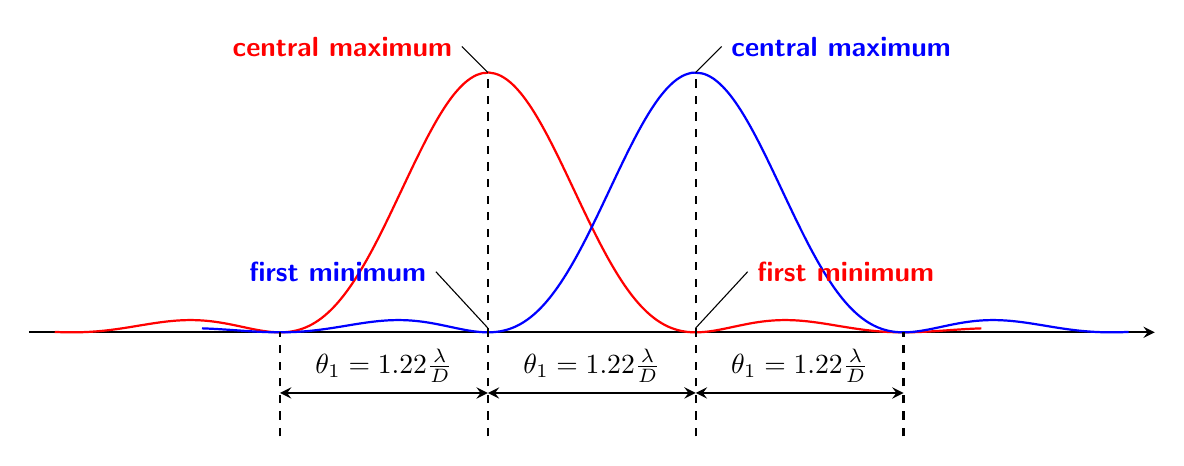
\begin{tikzpicture}[
    scale=1.1,
    >=stealth,
    declare function={
        sinc(\x) = (\x==0 ? 1 : sin(deg(\x))/\x);
    }
]

    % Geometry Parameters
    % Red peak at x = -1.2, Blue peak at x = 1.2
    % Peak separation alpha = theta_1 = 2.4 units (Rayleigh Criterion)
    \def\xR{-1.2}
    \def\xB{1.2}
    \def\dx{2.4} 

    % Base axis line
    \draw[->, thick] (-6.5,0) -- (6.5,0);

    % Red diffraction pattern: I(x) = (sinc(pi*(x - xR)/dx))^2
    \draw[red, thick, domain=-6.2:4.5, samples=300, smooth] 
        plot (\x, {3.0 * pow(sinc(3.14159 * (\x - \xR) / \dx), 2)});

    % Blue diffraction pattern: I(x) = (sinc(pi*(x - xB)/dx))^2
    \draw[blue, thick, domain=-4.5:6.2, samples=300, smooth] 
        plot (\x, {3.0 * pow(sinc(3.14159 * (\x - \xB) / \dx), 2)});

    % Vertical dashed lines
    \draw[dashed, thick] (\xR, -1.2) -- (\xR, 3.0);
    \draw[dashed, thick] (\xB, -1.2) -- (\xB, 3.0);
    \draw[dashed, thick] ({\xR - \dx}, -1.2) -- ({\xR - \dx}, 0);
    \draw[dashed, thick] ({\xB + \dx}, -1.2) -- ({\xB + \dx}, 0);

    % Bottom arrows explicitly labeling theta_1 = 1.22 lambda / D
    \draw[<->, thick] ({\xR - \dx}, -0.7) -- node[above] {$\theta_1 = 1.22 \frac{\lambda}{D}$} (\xR, -0.7);
    \draw[<->, thick] (\xR, -0.7) -- node[above] {$\theta_1 = 1.22 \frac{\lambda}{D}$} (\xB, -0.7);
    \draw[<->, thick] (\xB, -0.7) -- node[above] {$\theta_1 = 1.22 \frac{\lambda}{D}$} ({\xB + \dx}, -0.7);

    % Labels and pointer lines
    % Red central maximum label
    \draw[thin] (-1.5, 3.3) -- (\xR, 3.0);
    \node[red, font=\bfseries\sffamily, left] at (-1.5, 3.3) {central maximum};

    % Blue central maximum label
    \draw[thin] (1.5, 3.3) -- (\xB, 3.0);
    \node[blue, font=\bfseries\sffamily, right] at (1.5, 3.3) {central maximum};

    % Blue first minimum label (coincident with Red central peak)
    \draw[thin] (-1.8, 0.7) -- (\xR, 0.05);
    \node[blue, font=\bfseries\sffamily, left] at (-1.8, 0.7) {first minimum};

    % Red first minimum label (coincident with Blue central peak)
    \draw[thin] (1.8, 0.7) -- (\xB, 0.05);
    \node[red, font=\bfseries\sffamily, right] at (1.8, 0.7) {first minimum};

    \end{tikzpicture}
    \caption{Diffraction patterns of two barely resolved point sources under the Rayleigh criterion, where the central maximum of one source coincides with the first minimum ($\theta_1 = 1.22\lambda/D$) of the second.}
    \label{fig:rayleigh_diffraction_sinc}
\end{figure}

\begin{figure}[htbp]
    \centering
    
\includegraphics[width=0.6\linewidth]{Diffraction.pdf}
    \caption{Ray optics focusing through a circular entrance pupil and the resulting rotated Airy diffraction profile in the focal plane.}
    \label{fig:diffraction_pdf_diagram}
\end{figure}

\begin{example}[Diffraction Resolution at $\lambda = 500\,\mathrm{nm}$]
	For an optical telescope with aperture $D = 0.30\,\mathrm{m}$ observing at $\lambda = 500\,\mathrm{nm} = 500 \times 10^{-9}\,\mathrm{m}$:
	\[
	\theta_{\rm diff} = 1.22\frac{500 \times 10^{-9}}{0.30} \times \frac{180 \times 3600}{\pi}'' \simeq 2.03 \times 10^{-6} \times 206265'' = 0.42''.
	\]
\end{example}

\section{Comparing Pixel Scale to the Diffraction Limit: Nyquist Sampling}

\subsection{The Nyquist Sampling Criterion}

To record all spatial information contained in the image without aliasing, the \textbf{Nyquist sampling criterion} requires:
\begin{keyresult}
	\begin{equation}
		\text{Pixel Scale} \le \frac{\theta_{\rm res}}{2}.
		\label{eq:nyquist_sampling_criterion}
	\end{equation}
\end{keyresult}
That is, there must be at least \textbf{two detector pixels across the resolution element} ($\mathrm{FWHM} \approx \theta_{\rm res}$).

\subsection{Configuration Critique: Comparison of Pixel Scale and Diffraction Limit}

In the telescope configuration analyzed above:
\begin{itemize}
	\item The pixel scale is:
	\[
	\text{Pixel Scale} = \frac{y}{F}\bigg\lvert_{y=p} = 2.06''/\mathrm{pixel}.
	\]
	\item The diffraction-limited resolution is:
	\[
	\theta_{\rm res} = 1.22\frac{\lambda}{D} = 0.42''.
	\]
\end{itemize}
The Nyquist sampling criterion requires:
\[
\text{Pixel Scale} \le \frac{\theta_{\rm res}}{2} = \frac{0.42''}{2} = 0.21'',
\]
which is \textbf{not respected}. 

Evaluating the ratio of the two quantities:
\begin{keyresult}
	\begin{equation}
		\frac{\text{Pixel Scale}}{\theta_{\rm res}} = \frac{2.06}{0.42} \simeq 4.9.
		\label{eq:pixel_diffraction_ratio}
	\end{equation}
\end{keyresult}
Thus, \textbf{one pixel covers almost five diffraction-limited resolution elements}, which represents a severely \emph{undersampled} configuration. High spatial frequencies are permanently lost to digital aliasing, and point sources cannot be astrometrically centroided to sub-diffraction accuracy.

\begin{table}[htbp]
	\centering
	\small
	\begin{tabular}{lp{5.5cm}p{6.0cm}}
		\toprule
		\textbf{Sampling Regime} & \textbf{Condition} & \textbf{Observational Consequences} \\
		\midrule
		\textbf{Critically Sampled} & $\text{Pixel Scale} \approx \theta_{\rm res}/2$ & Preserves all spatial frequencies without wasting detector area. \\
		\textbf{Undersampled} & $\text{Pixel Scale} > \theta_{\rm res}/2$ & Causes aliasing, jagged stellar profiles, and astrometric centroid degradation. \\
		\textbf{Oversampled} & $\text{Pixel Scale} \ll \theta_{\rm res}/2$ & Spreads light over excessive pixels, increasing total readout noise penalty $\sqrt{n_{\rm pix}}\sigma_{\rm RON}$. \\
		\bottomrule
	\end{tabular}
	\caption{Comparison of digital detector sampling regimes in astronomical imaging.}
	\label{tab:sampling_regimes}
\end{table}

\section{Atmospheric Seeing, PSF Profiles, and Adaptive Optics}

\subsection{Atmospheric Seeing and the Fried Parameter ($r_0$)}

For ground-based optical telescopes, turbulent temperature and density variations in the Earth's atmosphere distort incoming plane wavefronts. The spatial scale over which wavefront phases remain coherent is parameterized by the \textbf{Fried coherence parameter} $r_0$ (typically $r_0 \sim 10\text{--}20\,\mathrm{cm}$ in the $V$-band at premier mountain observatories).

For any telescope with aperture diameter $D > r_0$, the delivered angular resolution is limited not by $D$, but by $r_0$:
\begin{keyresult}
	\begin{equation}
		\theta_{\rm seeing} \approx 0.98\frac{\lambda}{r_0} \sim 0.5''\text{--}1.5''.
		\label{eq:seeing_resolution}
	\end{equation}
\end{keyresult}
Because $r_0 \propto \lambda^{6/5}$, seeing improves at infrared wavelengths ($\theta_{\rm seeing} \propto \lambda^{-1/5}$).

\subsection{Point Spread Function (PSF) Profiles: The Moffat Function}

Turbulent atmospheric scattering smears the theoretical Airy disk into a broader Point Spread Function (PSF). Astronomers parameterize this profile using the \textbf{Moffat function}:
\begin{equation}
	I(r) = I_0 \left[1 + \left(\frac{r}{\alpha}\right)^2\right]^{-\beta}, \qquad \mathrm{FWHM} = 2\alpha\sqrt{2^{1/\beta}-1},
	\label{eq:moffat_function}
\end{equation}
where $\beta \approx 2.5\text{--}4.5$ captures the extended scattering wings produced by Kolmogorov turbulence.

\subsection{Adaptive Optics (AO)}

Adaptive Optics systems restore diffraction-limited performance to ground-based telescopes in real time:
\begin{enumerate}
	\item A \textbf{Wavefront Sensor} (e.g., Shack--Hartmann lenslet array) measures instantaneous phase distortions $\Delta\phi(\mathbf r, t)$ at kHz frequencies using a bright Natural Guide Star (NGS) or Sodium Laser Guide Star (LGS, $\lambda = 589\,\mathrm{nm}$ resonant excitation at $\sim 90\,\mathrm{km}$ altitude).
	\item A real-time computer calculates the required phase conjugation.
	\item A \textbf{Deformable Mirror} (with hundreds to thousands of piezoelectric actuators) physically adjusts its surface profile to cancel out the atmospheric optical path difference.
\end{enumerate}
This restores the sharp $\theta \approx \lambda/D$ diffraction core on 8--30 meter class telescopes, providing space-quality resolution from the ground.
